\section{Implementation Details}\label{sec:impl_details}
So far we have discussed our high level ideas for implementing an efficient multisplit algorithm for GPUs. In this section we thoroughly describe our design choices and implementation details.
We first discuss existing memory and computational hierarchies in GPUs, and conventional localization options available on such devices.
Then we discuss traditional design choices for similar problems such as multisplit, histogram, and radix sort.
We follow this by our own design choices and how they differ from previous work.
Finally, we propose three implementation variations of multisplit, each with its own localization method and computational details.

\subsection{GPU memory and computational hierarchies}\label{subsec:gpu_hierarchy}
As briefly discussed in Section~\ref{sec:related}, GPUs offer three main memory storage options: 1)~registers dedicated to each thread, 2)~shared memory dedicated to all threads within a thread-block, 3)~global memory accessible by all threads in the device.\footnote{There are other types of memory units in GPUs as well, such as local, constant, and texture memory. However, these are in general special-purpose memories and hence we have not targeted them in our design.}
From a computational point of view there are two main computational units: 1)~threads have direct access to arithmetic units and perform register-based computations, 2)~all threads within a warp can perform a limited but useful set of hardware based warp-wide intrinsics (e.g., ballots, shuffles, etc.). Although the latter is not physically a new computational unit, its inter-register communication among threads opens up new computational capabilities (such as parallel voting).

Based on memory and computational hierarchies discussed above, there are four primary ways of solving a problem on the GPU: 1)~thread-level, 2)~warp-level, 3)~block-level, and 4)~device-level (global).
Traditionally, most efficient GPU programs for multisplit, histogram and radix sort~\cite{He:2008:RJG, Bell:2011:TAP, Merrill:2015:CUB} start from  thread-level computations, where each thread processes a group of input elements and performs local computations (e.g., local histograms).
These thread-level results are then usually combined to form a block-level solution, usually to benefit from the block's shared memory.
Finally, block-level results are combined together to form a global solution.
If implemented efficiently, these methods are capable of achieving high-quality performance from available GPU resources (e.g., CUB's high efficiency in histogram and radix sort).

In contrast, we advocate another way of solving these problems, based on a warp granularity. We start from a warp-level solution and then proceed up the hierarchy to form a device-wide (global) solution (we may bypass the block-level solution as well).
Consequently, we target two major implementation alternatives to solve our multisplit problem: 1)~warp-level~$\rightarrow$ device-level, 2)~warp-level~$\rightarrow$ block-level~$\rightarrow$ device-level
(in Section~\ref{subsec:ms_privatization}, we discuss the costs and benefits of our approaches compared to a thread-level approach).
Another algorithmic option that we outlined in Section~\ref{subsec:alg_reordering} was to reorder elements to get better (coalesced) memory accesses.
As a result of combining these two sets of alternatives, there will be four possible variations that we can explore.
However, if we neglect reordering, our block-level solution will be identical to our warp-level solution, which leaves us with three main final options that all start with warp-level subproblem solutions and end up with a device-level global solution: 1)~no reordering, 2)~with reordering and bypassing a block-level solution, 3)~with reordering and including a block-level solution.
Next, we describe these three implementations and show how they fit into the multi-level localization model we described in Section~\ref{subsec:localization}.

\subsection{Our proposed multisplit algorithms}
So far we have seen that we can reduce the size and cost of our global operation (size of $\mathbf{H}$) by doing more local work (based on our multi-level localization and hierarchical approach). This is a complex tradeoff, since we prefer a small number of subproblems in our first level (global operations), as well as small enough subproblem sizes in our last levels so that they can easily be solved within a warp.
What remains is to choose the number and size of our localization levels and where to perform reordering. All these design choices should be made based on a set of complicated factors such as available shared memory and registers, achieved occupancy, required computational load, etc.

In this section we describe three novel and efficient multisplit implementations that explore different points in the design space, using the terminology that we introduced in Section~\ref{subsec:localization} and Section~\ref{subsec:gpu_hierarchy}.

\begin{description}
\item[Direct Multisplit] Rather than split the problem into subproblems across threads, as in traditional approaches~\cite{He:2008:RJG}, Direct Multisplit (DMS) splits the problem into subproblems across warps (warp-level approach), leveraging efficient warp-wide intrinsics to perform the local computation.
\item[Warp-level Multisplit] Warp-level Multisplit (WMS) also uses a warp-level approach, but additionally reorders elements within each subproblem for better locality.
\item[Block-level Multisplit] Block-level Multisplit (BMS) modifies WMS to process larger-sized subproblems with a block-level approach that includes reordering, offering a further reduction in the cost of the global step at the cost of considerably more complex local computations.
\end{description}

We now discuss the most interesting aspects of our implementations of these three approaches, separately describing how we divide the problem into smaller pieces (our localization strategies), compute histograms and local offsets for larger subproblem sizes, and reorder final results before writing them to global memory to increase coalescing.
% We begin this section by our novel voting strategy which becomes a cornerstone in all our computations. Then we gradually make our design more complete as we follow through this section.
%%%%%%%%%%%%%%%%%%%%%%%%%%%%%%%%%%%%%%%%%%%%%%%%%%%%%%%%%%%%%%%%%%%
\subsection{Localization and structure of our multisplit}\label{subsec:ms_localization}
In Section~\ref{sec:algorithm} we described our parallel model in solving the multisplit problem.
Theoretically, we would like to both minimize our global computations as well as maximize our hardware utilization.
However, in practice designing an efficient GPU algorithm is more complicated.
There are various factors that need to be considered, and sometimes even be smartly sacrificed in order to satisfy a more important goal: efficiency of the whole algorithm.
For example, we may decide to recompute the same value multiple times in different kernel launches, just so that we do not need to store them in global memory for further reuse.

In our previous work~\cite{Ashkiani:2016:GM}, we implemented our multisplit algorithms with a straightforward localization strategy: Direct and Warp-level Multisplit divided problems into warp-sized subproblems (two levels of localization), and Block-level Multisplit used block-sized subproblems (three levels of localization) to extract more locality by performing more complicated computations needed for reordering.
In order to have better utilization of available resources, we assigned multiple similar tasks to each launched warp/block (so each warp/block processed multiple independent subproblems).
Though this approach was effective, we still faced relatively expensive global computations, and did not extract enough locality from our expensive reordering step.
Both of these issues could be remedied by using larger subproblems within the same localization hierarchy. However, larger subproblems require more complicated computations and put more pressure on the limited available GPU resources (registers, shared memory, memory bandwidth, etc.). Instead, we redesigned our implementations to increase the number of levels of localization. This lets us have larger subproblems, while systematically coordinating our computational units (warps/blocks) and available resources to achieve better results.

\paragraph{Direct Multisplit} Our DMS implementation has three levels of localizations: 
Each warp is assigned to a chunk of consecutive elements (first level).
This chunk is then divided into a set of consecutive windows of warp-width ($N_\text{thread}=32$) size (second level).
For each window, we multisplit without any reordering (third level).
\paragraph{Warp-level Multisplit} WMS is similar to DMS, but it also performs reordering to get better locality. In order to get better resource utilization, we add another level of localization compared to DMS (total of four). Each warp performs reordering over only a number of processed windows (a \emph{tile}), and then continues to process the next tile. In general, each warp is in charge of a chunk of consecutive elements (first level). Each chunk is divided into several consecutive tiles (second level). Each tile is processed by a single warp and reordered by dividing it into several consecutive windows (third level). Each window is then directly processed by warp-wide methods (fourth level).
The reason that we add another level of localization for each tile is simply because we do not have sufficient shared memory per warp to store the entire subproblem.

\paragraph{Block-level Multisplit} BMS has five levels of localization. Each thread-block is in charge of a chunk of consecutive elements (first level). Each chunk is divided into a consecutive number of tiles (second level). Each tile is processed by all warps within a block (third level) and reordering happens in this level. Each warp processes multiple consecutive windows of input data within the tile (fourth level). In the end each window is processed directly by using warp-wide methods (fifth level). Here, for a similar reason as in WMS (limited shared memory), we added another level of localization per tile.

Figure~\ref{fig:multisplit_levels} shows a schematic example of our three methods next to each other. Note that we have flexibility to tune subproblem sizes in each implementation by changing the sizing parameters in Table~\ref{table:subproblems}.

\begin{table}
\centering
\small
\begin{tabular}{ll}
\toprule
Algorithm & subproblem size ($\bar{n}$) \\
\midrule
DMS     & $N_\text{(window/warp)}N_\text{thread}$ \\
WMS     & $N_\text{(tile/warp)}N_\text{(window/tile)}N_\text{thread}$ \\
BMS     & $N_\text{(tile/block)}N_\text{(warp/tile)}N_\text{(window/warp)}N_\text{thread}$ \\
\bottomrule
\end{tabular}
\caption{Size of subproblems for each multisplit algorithm. Total size of our global computations will then be the size of $\mathbf{H}$ equal to $mn/\bar{n}$.}\label{table:subproblems}
\end{table}

\begin{figure}
  \centering

  \begin{tabular}{ccc}
  \subfloat[DMS localization]{
          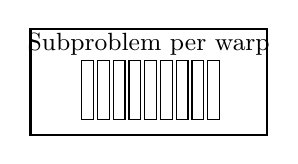
\begin{tikzpicture}[every node/.style={thick,rectangle,inner sep=0pt}]

\def \dx {0.05}
\def \dy {0.2}
\def \recx {0.15}
\def \recX {9*\recx + 10*\dx}
\def \recy {0.75}
\def \recY {\recy + 3 * \dy}

%% left child 
\draw [black] (0 + 0, 0 + 0) rectangle (0 + \recx, 0 + \recy);
\draw [black] (0 + \recx + \dx, 0) rectangle (0 + 2*\recx + \dx, 0 + \recy);
\draw [black] (0 + 2*\recx + 2*\dx, 0 + 0) rectangle (0 + 3*\recx + 2*\dx, 0 + \recy);
\draw [black] (0 + 3*\recx + 3*\dx, 0 + 0) rectangle (4*\recx + 3*\dx, 0 + \recy);
\draw [black] (0 + 4*\recx + 4*\dx, 0 + 0) rectangle (5*\recx + 4*\dx, 0 + \recy);
\draw [black] (0 + 5*\recx + 5*\dx, 0 + 0) rectangle (6*\recx + 5*\dx, 0 + \recy);
\draw [black] (0 + 6*\recx + 6*\dx, 0 + 0) rectangle (7*\recx + 6*\dx, 0 + \recy);
\draw [black] (0 + 7*\recx + 7*\dx, 0 + 0) rectangle (8*\recx + 7*\dx, 0 + \recy);
\draw [black] (0 + 8*\recx + 8*\dx, 0 + 0) rectangle (9*\recx + 8*\dx, 0 + \recy);

\draw[thick, black] (0-13*\dx, 0-\dy) rectangle (0-13*\dx + \recX + 23 * \dx, 0-\dy + \recY);
\node () at (0 + 5 * \recx + 2 * \dx, \recy + \dy) {\small Subproblem per warp};

\end{tikzpicture}
  } &
  \subfloat[WMS localization]{
                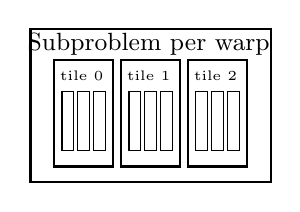
\begin{tikzpicture}[every node/.style={thick,rectangle,inner sep=0pt}]

\def \dx {0.05}
\def \dy {0.2}
\def \recx {0.15}
\def \recX {3*\recx + 4*\dx}
\def \recXX {3 * \recX + 22 * \dx}
\def \recy {0.75}
\def \recY {\recy + 3 * \dy}
\def \recYY {\recY + 3 * \dy}

%% left child 
\draw [black] (0 + 0, 0 + 0) rectangle (0 + \recx, 0 + \recy);
\draw [black] (0 + \recx + \dx, 0) rectangle (0 + 2*\recx + \dx, 0 + \recy);
\draw [black] (0 + 2*\recx + 2*\dx, 0 + 0) rectangle (0 + 3*\recx + 2*\dx, 0 + \recy);

\draw[thick, black] (0-2*\dx, 0-\dy) rectangle (0-2*\dx + \recX + 2 * \dx, 0-\dy + \recY);
\node () at (0 + 1 * \recx + 2 * \dx, \recy + \dy) {\tiny tile 0};

\draw [black] (\recX + 4*\dx + 0, 0 + 0) rectangle (\recX + 4*\dx + \recx, 0 + \recy);
\draw [black] (\recX + 4*\dx + \recx + \dx, 0) rectangle (\recX + 4*\dx + 2*\recx + \dx, 0 + \recy);
\draw [black] (\recX + 4*\dx + 2*\recx + 2*\dx, 0 + 0) rectangle (\recX + 4*\dx + 3*\recx + 2*\dx, 0 + \recy);

\draw[thick, black] (\recX + 4*\dx-2*\dx, 0-\dy) rectangle (\recX + 4*\dx-2*\dx + \recX + 2 * \dx, 0-\dy + \recY);
\node () at (\recX + 4*\dx + 1 * \recx + 2 * \dx, \recy + \dy) {\tiny tile 1};

\draw [black] (2*\recX + 12*\dx + 0, 0 + 0) rectangle (2*\recX + 12*\dx + \recx, 0 + \recy);
\draw [black] (2*\recX + 12*\dx + \recx + \dx, 0) rectangle (2*\recX + 12*\dx + 2*\recx + \dx, 0 + \recy);
\draw [black] (2*\recX + 12*\dx + 2*\recx + 2*\dx, 0 + 0) rectangle (2*\recX + 12*\dx + 3*\recx + 2*\dx, 0 + \recy);

\draw[thick, black] (2*\recX + 12*\dx-2*\dx, 0-\dy) rectangle (2*\recX + 12*\dx-2*\dx + \recX + 2 * \dx, 0-\dy + \recY);
\node () at (2*\recX + 12*\dx + 1 * \recx + 2 * \dx, \recy + \dy) {\tiny tile 2};

\draw [thick, black] (0-8*\dx, 0-2*\dy) rectangle (0 + \recXX, 0-2*\dy + \recYY);
\node () at (\recX + 4*\dx + 1 * \recx + 2 * \dx, \recy + 3* \dy) {\small Subproblem per warp};

% \def\dx{1}
% \def\a{0}
% \def\recx{0.15}
% \def\recy{0.75}
% \def \recyTile{2*\recy}
% \def \recxTile{5*\recx}
% \def \recxSubp{4 * \recxTile}
% \def \recySubp{1.5 * \recyTile}

% \node (a1) at (0 * \dx,0) [draw, minimum width=\recx cm, minimum height=\recy cm, anchor=north] {};
% \node (a2) [right=2pt of a1, draw=black,rectangle,minimum width = \recx cm, minimum height=\recy cm] {};
% \node (a3) [right=2pt of a2, draw=black,rectangle,minimum width = \recx cm, minimum height=\recy cm] {};
% \node (t1) [above=1pt of a2, anchor=south] {};

% \node (b1) [draw, fit=(a1)(a2)(a3)(t1), label={\scriptsize tile 0}, minimum width = \recxTile cm, minimum height=\recyTile cm] {};

% \node (a4) at (1 * \dx,0) [draw, minimum width=\recx cm, minimum height=\recy cm, anchor=north] {};
% \node (a5) [right=2pt of a4, draw=black,rectangle,minimum width = \recx cm, minimum height=\recy cm] {};
% \node (a6) [right=2pt of a5, draw=black,rectangle,minimum width = \recx cm, minimum height=\recy cm] {};
% \node (t4) [above=1pt of a5, anchor=south] {};

% \node (b4) [draw, fit=(a4)(a5)(a6)(t4), label={\scriptsize tile 1}, minimum width = \recxTile cm, minimum height=\recyTile cm] {};

% \node (a7) at (2 * \dx,0) [draw, minimum width=\recx cm, minimum height=\recy cm, anchor=north] {};
% \node (a8) [right=2pt of a7, draw=black,rectangle,minimum width = \recx cm, minimum height=\recy cm] {};
% \node (a9) [right=2pt of a8, draw=black,rectangle,minimum width = \recx cm, minimum height=\recy cm] {};
% \node (t7) [above=1pt of a8, anchor=south] {};

% \node (b7) [draw, fit=(a7)(a8)(a9)(t7), label={\scriptsize tile 2}, minimum width = \recxTile cm, minimum height=\recyTile cm] {};

% \node (c1) [draw, fit=(b7)(b4)(b1), label={\small Subproblem per warp}, minimum width = \recxSubp cm, minimum height=\recySubp cm] {};
\end{tikzpicture}
  } &
  \subfloat[BMS localization]{
                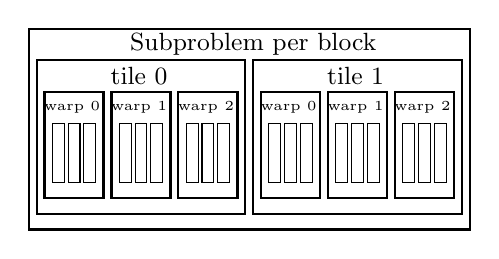
\begin{tikzpicture}[every node/.style={thick,rectangle,inner sep=0pt}]
\def \dx {0.05}
\def \dy {0.2}
\def \recx {0.15}
\def \recX {3*\recx + 4*\dx}
\def \recXX {3 * \recX + 22 * \dx}
\def \recy {0.75}
\def \recY {\recy + 3 * \dy}
\def \recYY {\recY + 3 * \dy}

%% left child 
\draw [black] (0 + 0, 0 + 0) rectangle (0 + \recx, 0 + \recy);
\draw [black] (0 + \recx + \dx, 0) rectangle (0 + 2*\recx + \dx, 0 + \recy);
\draw [black] (0 + 2*\recx + 2*\dx, 0 + 0) rectangle (0 + 3*\recx + 2*\dx, 0 + \recy);

\draw[thick, black] (0-2*\dx, 0-\dy) rectangle (0-2*\dx + \recX + 2 * \dx, 0-\dy + \recY);
\node () at (0 + 1 * \recx + 2 * \dx, \recy + \dy) {\tiny warp 0};

\draw [black] (\recX + 4*\dx + 0, 0 + 0) rectangle (\recX + 4*\dx + \recx, 0 + \recy);
\draw [black] (\recX + 4*\dx + \recx + \dx, 0) rectangle (\recX + 4*\dx + 2*\recx + \dx, 0 + \recy);
\draw [black] (\recX + 4*\dx + 2*\recx + 2*\dx, 0 + 0) rectangle (\recX + 4*\dx + 3*\recx + 2*\dx, 0 + \recy);

\draw[thick, black] (\recX + 4*\dx-2*\dx, 0-\dy) rectangle (\recX + 4*\dx-2*\dx + \recX + 2 * \dx, 0-\dy + \recY);
\node () at (\recX + 4*\dx + 1 * \recx + 2 * \dx, \recy + \dy) {\tiny warp 1};

\draw [black] (2*\recX + 12*\dx + 0, 0 + 0) rectangle (2*\recX + 12*\dx + \recx, 0 + \recy);
\draw [black] (2*\recX + 12*\dx + \recx + \dx, 0) rectangle (2*\recX + 12*\dx + 2*\recx + \dx, 0 + \recy);
\draw [black] (2*\recX + 12*\dx + 2*\recx + 2*\dx, 0 + 0) rectangle (2*\recX + 12*\dx + 3*\recx + 2*\dx, 0 + \recy);

\draw[thick, black] (2*\recX + 12*\dx-2*\dx, 0-\dy) rectangle (2*\recX + 12*\dx-2*\dx + \recX + 2 * \dx, 0-\dy + \recY);
\node () at (2*\recX + 12*\dx + 1 * \recx + 2 * \dx, \recy + \dy) {\tiny warp 2};

\draw [thick, black] (0-4*\dx, 0-2*\dy) rectangle (0-4*\dx + \recXX, 0-2*\dy + \recYY);
\node () at (\recX + 4*\dx + 1 * \recx + 2 * \dx, \recy + 3* \dy) {\small tile 0};

%% right child
\draw [black] (\recXX + 2*\dx + 0, 0 + 0) rectangle (\recXX +2*\dx+ \recx, 0 + \recy);
\draw [black] (\recXX + 2*\dx + \recx + \dx, 0) rectangle (\recXX +2*\dx+ 2*\recx + \dx, 0 + \recy);
\draw [black] (\recXX + 2*\dx + 2*\recx + 2*\dx, 0 + 0) rectangle (\recXX +2*\dx+ 3*\recx + 2*\dx, 0 + \recy);

\draw[thick, black] (\recXX, 0-\dy) rectangle (\recXX + \recX + 2 * \dx, 0-\dy + \recY);
\node () at (\recXX + 2*\dx +  1 * \recx + 2 * \dx, \recy + \dy) {\tiny warp 0};

\draw [black] (\recXX + 2*\dx+\recX + 4*\dx + 0, 0 + 0) rectangle (\recXX + 2*\dx+\recX + 4*\dx + \recx, 0 + \recy);
\draw [black] (\recXX + 2*\dx+\recX + 4*\dx + \recx + \dx, 0) rectangle (\recXX + 2*\dx+\recX + 4*\dx + 2*\recx + \dx, 0 + \recy);
\draw [black] (\recXX + 2*\dx+\recX + 4*\dx + 2*\recx + 2*\dx, 0 + 0) rectangle (\recXX + 2*\dx+\recX + 4*\dx + 3*\recx + 2*\dx, 0 + \recy);

\draw[thick, black] (\recXX + 2*\dx+\recX + 4*\dx-2*\dx, 0-\dy) rectangle (\recXX + 2*\dx+\recX + 4*\dx-2*\dx + \recX + 2 * \dx, 0-\dy + \recY);
\node () at (\recXX + 2*\dx+\recX + 4*\dx + 1 * \recx + 2 * \dx, \recy + \dy) {\tiny warp 1};

\draw [black] (\recXX + 2*\dx + 2*\recX + 12*\dx + 0, 0 + 0) rectangle (\recXX + 2*\dx + 2*\recX + 12*\dx + \recx, 0 + \recy);
\draw [black] (\recXX + 2*\dx + 2*\recX + 12*\dx + \recx + \dx, 0) rectangle (\recXX + 2*\dx + 2*\recX + 12*\dx + 2*\recx + \dx, 0 + \recy);
\draw [black] (\recXX + 2*\dx + 2*\recX + 12*\dx + 2*\recx + 2*\dx, 0 + 0) rectangle (\recXX + 2*\dx + 2*\recX + 12*\dx + 3*\recx + 2*\dx, 0 + \recy);

\draw[thick, black] (\recXX + 2*\dx + 2*\recX + 12*\dx-2*\dx, 0-\dy) rectangle (\recXX + 2*\dx + 2*\recX + 12*\dx-2*\dx + \recX + 2 * \dx, 0-\dy + \recY);
\node () at (\recXX + 2*\dx + 2*\recX + 12*\dx + 1 * \recx + 2 * \dx, \recy + \dy) {\tiny warp 2};

\draw [thick, black] (\recXX-2*\dx, 0-2*\dy) rectangle (\recXX-2*\dx + \recXX, 0-2*\dy + \recYY);
\node () at (\recXX  + 2*\dx + \recX + 4*\dx + 1 * \recx + 2 * \dx, \recy + 3* \dy) {\small tile 1};

%% subproblem per block:
\draw [thick, black] (0-6*\dx, 0 - 3 * \dy) rectangle (0-6*\dx + 3*\recXX + 5*\dx, 0-3*\dy + \recYY + 3*\dy);
\node () at (\recXX -2* \dx, \recYY -\dy) {\small Subproblem per block};
\end{tikzpicture}
  }
  \end{tabular}
  \caption{Different localizations for DMS, WMS and BMS are shown schematically. Assigned indices are just for illustration. Each small rectangle denotes a window of 32 consecutive elements. Reordering takes place per tile, but global offsets are computed per subproblem. \label{fig:multisplit_levels}}
\end{figure}

Next we briefly highlight the general structure of our computations (based on our model in Section~\ref{subsec:parallel_model}). We use DMS to illustrate:

\paragraph{Pre-scan (local)} Each warp reads a window of key elements (of size $N_\text{thread} = 32$), generates a local matrix $\bar{\mathbf{H}}$, and computes its histogram (reducing each row). Next, histogram results are stored locally in registers. Then, each warp continues to the next window and repeats the process, adding histogram results to the results from previous windows.
In the end, each warp has computed a single column of $\mathbf{H}$ and stores its results into global memory.
\paragraph{Scan (global)} We perform an exclusive scan operation over the row-vectorized $\mathbf{H}$ and store the result back into global memory (e.g., matrix $\mathbf{G} = [g_{i,\ell}]_{m\times L_0}$).
\paragraph{Post-scan (local)} Each warp reads a window of key-value pairs, generates its local matrix $\bar{\mathbf{H}}$ again,\footnote{Note that we compute $\bar{\mathbf{H}}$ a second time rather than storing and reloading the results from the computation in the first step. This is deliberate. We find that the recomputation is cheaper than the cost of global store and load.} and computes local offsets (with a local exclusive scan on each row).
Similar to the pre-scan stage, we store histogram results into registers.
We then compute final positions by using the global base addresses from $\mathbf{G}$, warp-wide base addresses (warp-wide histogram results up until that window), and local offsets. Then we write key-value pairs directly to their storage locations in the output vector. For example, if key $u \in B_i$ is read by warp $\ell$ and its local offset is equal to $k$, its final position will be $g_{i,\ell} + h_i + k$, where $h_i$ is the warp-wide histogram result up until that window (referring to equation~\eqref{eq:permutation3} is helpful to visualize how we compute final addresses with a multi-level localization).

Algorithm~\ref{alg:dms} shows a simplified pseudo-code of the DMS method (with less than 32 buckets). Here, we can identify each key's bucket by using a \texttt{bucket\_identifier()} function. We compute warp histogram and local offsets with \texttt{warp\_histogram()} and \texttt{warp\_offsets()} procedures, which we describe in detail later in this section (Alg.~\ref{alg:warp_histogram}~and~\ref{alg:warp_offsets}).

\begin{algorithm}
\KwIn {\text{key\_in[]}, \text{value\_in[]}, \text{bucket\_identifier()}: keys, values and a bucket identifier function.}
\KwOut {\text{key\_out[]}, \text{value\_out[]}: keys and values after multisplit.}
// {key\_in[], value\_in[], key\_out[], value\_out[], H, and G are all stored in global memory.}
// {L: number of subproblems}

// {\bf ====== Pre-scan stage:}

\For{each warp \textnormal{i=0:L-1} {\bf parallel device}}{
        histo[0:m-1] = 0\;
        \For{each window \textnormal{j=0:N\_window-1}}{
    \text{bucket\_id[0:31] = \text{bucket\_identifier(key\_in[32*i*N\_window + 32*j + (0:31)])\;}}

    \text{histo[0:m-1]} += \text{warp\_histogram(bucket\_id[0:31])\;}
  }
  \text{H[0:m-1][i] = histo[0:m-1]\;}
}

// {\bf ====== Scan stage:}

\text{H\_row = [H[0][0:L-1],H[1][0:L-1], \ldots, H[m-1][0:L-1]]\;}

\text{G\_row = exclusive\_scan(H\_row)\;}

// \text{[G[0][0:L-1],G[1][0:L-1], \ldots, G[m-1][0:L-1]] = G\_row\;}

\For{\textnormal{i = 0:m-1} and \textnormal{j = 0:L-1}}{
  G[i][j] = \text{G\_row[i $\ast$ m + j]\;}
}

// {\bf ====== Post-scan stage:}

\For {each warp \textnormal{i=0:L-1} {\bf parallel device}}{
        histo[0:m-1] = 0\;
        \For{each window \textnormal{j=0:N\_window-1}}{
                read\_key = key\_in[32*i*N\_window + 32*j + (0:31)]\;
                read\_value = value\_in[32*i*N\_window + 32*j + (0:31)]\;
          \text{bucket\_id[0:31] = \text{bucket\_identifier(read\_key)\;}}

          \text{offsets[0:31]} = \text{warp\_offsets(bucket\_id[0:31])\;}

    \For{each thread \textnormal{k=0:31} {\bf parallel warp}}{
        \text{final\_position[k] = G[bucket\_id[k]][i] + histo[bucket\_id[k]] + offsets[k]\;}

        \text{key\_out[final\_position[k]] = read\_key\;}

        \text{value\_out[final\_position[k]] = read\_value\;}
    }

    \text{histo[0:m-1]} += \text{warp\_histogram(bucket\_id[0:31])\;} // \emph{updating histograms}    
  }
}
\caption{The Direct Multisplit (DMS) algorithm}\label{alg:dms}
\end{algorithm}

%%%%%%%%%%%%%%%%%%%%%%%%%%%%%%%%%%%%%%%%%%%%%%%%%%%%%%%%%%%%%%%%%%%
\subsection{Ballot-based voting}\label{subsec:ballot}
In this section, we momentarily change our direction into exploring a theoretical problem about voting.
We then use this concept to design and implement our warp-wide histograms (Section~\ref{subsec:histogram}).
We have previously emphasized our design decision of a warp-wide granularity. This decision is enabled by the efficient warp-wide intrinsics of NVIDIA GPUs.
In particular, NVIDIA GPUs support a warp-wide intrinsic \texttt{\_\_ballot(predicate)}, which performs binary voting across all threads in a warp. More specifically, each thread evaluates a local Boolean predicate, and depending on the result of that predicate (true or false), it toggles a specific bit corresponding to its position in the warp (i.e., lane ID from 0 to 31).
With a 32-element warp, this ballot fits in a 32-bit register, so that the $i$th thread in a warp toggles the $i$th bit.
After the ballot is computed, every participant thread can access the ballot result (as a bitmap) and see the voting result from all other threads in the same warp.

Now, the question we want to answer within our multisplit implementation is a generalization to the voting problem: Suppose there are $m$ arbitrary agents (indexed from $0$ to $n-1$), each evaluating a personalized non-binary predicate (a vote for a candidate) that can be any value from $0$ to $m-1$. 
How is it possible to perform the voting so that any agent can know all the results (who voted for whom)?

A naive way to solve this problem is to perform $m$ separate binary votes. For each round $0 \leq i < m$, we just ask if anyone wants to vote for $i$. Each vote has a binary result (either voting for $i$ or not). After $m$ votes, any agent can look at the $m\times n$ ballots and know which agent voted for which of the $m$ candidates. 
% \john{Any particular reason why the number of agents needs to equal the number of candidates? I think those two things are separable.}

We note that each agent's vote ($0 \leq v_i < n$) can be represented by $\log m$ binary digits. So a more efficient way to solve this problem requires just $\log m$ binary ballots per agent. Instead of directly asking for a vote per candidate ($m$ votes/bitmaps), we can ask for consecutive bits of each agent's vote (a bit at a time) and store them as a bitmap (for a total of $\log m$ bitmaps, each bitmap of size $n$).
For the $j$th bitmap ($0 \leq j < \lceil\log m\rceil$), every $i$th bit is one if only the $i$th agent have voted to a candidate whose $j$th bit in its binary representation was also one (e.g., the 0th bitmap includes all agents who voted for an odd-numbered candidate).  
% \john{Seems like this is backwards: $\log m$ might be less than $j$, yeah? There's a ceil involved.} 
% contains a one for all those agents whose chosen candidate's $j$th bit was a one, and similarly for each zero.

As a result, these $\lceil \log m \rceil$ bitmaps together contain all information to reconstruct every agent's vote. All we need to do is to imagine each bitmap as a row of a $m\times n$ matrix.
Each column represent the binary representation of the vote of that specific agent. 
Next, we use this scheme to perform some of our warp-wide computations, only using NVIDIA GPU's binary ballots.
% Given these $j$ bitmaps, how do we compute a new bitmap $Y_i$ that shows only those who exactly voted for a particular agent $i$? Imagine each bitmap variable $X_j$ as a row in a binary matrix. In this matrix, each column $k$ denotes the binary representation of a candidate who was the choice of the $k$th agent. Thus, for each column, we can logically AND all binary elements including 1)~those that the corresponding bit in binary representation of $i$ is one, 2)~logical NOT of those otherwise. \john{This previous sentence doesn't make sense to me.}
%%%%%%%%%%%%%%%%%%%%%%%%%%%%%%%%%%%%%%%%%%%%%%%%%%%%%%%%%%%%%%%%%%%
\subsection{Computing Histograms and Local Offsets}\label{subsec:histogram}
The previous subsections described why and how we create a hierarchy of localizations. Now we turn to the problem of computing a direct solve of histograms and local offsets on a warp-sized (DMS or WMS) or a block-sized (BMS) problem. In our implementation, we leverage the balloting primitives we described in Section~\ref{subsec:ballot}.
We assume throughout this section that the number of buckets does not exceed the warp width ($m \leq N_\text{thread}$). Later we extend our discussion to any number of buckets in Section~\ref{subsec:more_buckets}.

\subsubsection{Warp-level Histogram}\label{subsubsec:warp_histogram}
Previously, we described our histogram computations in each subproblem as forming a binary matrix $\bar{\mathbf{H}}$ and doing certain computations on each row (reduction and scan).
Instead of explicitly forming the binary matrix $\bar{\mathbf{H}}$, each thread generates its own version of the rows of this matrix and stores it in its local registers as a binary bitmap. Then per-row reduction is equivalent to a population count operation (\texttt{\_\_popc}), and exclusive scan equates to first masking corresponding bits and then reducing the result. We now describe both in more detail.

To compute warp-level histograms, we assign each bucket (each row of $\bar{\mathbf{H}}$) to a thread. That thread is responsible for counting the elements of the warp (of the current read window of input keys) that fall into that bucket.
We described in Section~\ref{subsec:ballot} how each agent (here, each thread) can know about all the votes (here, the bucket to which each key belongs).
Since we assigned each thread to count the results of a particular bucket (here, the same as its lane ID ranging from 0 to 31), each thread must only count the number of other threads that voted for a bucket equal to its lane ID (the bucket to which it is assigned).
For cases where there are more buckets than the warp width, we assign $\lceil m/32 \rceil$ buckets to each thread.
First, we focus on $m\leq 32$; Algorithm~\ref{alg:warp_histogram} shows the detailed code.

\begin{algorithm}
\DontPrintSemicolon
% // {\emph{all threads within a warp}}.
\Fn{warp\_histogram(bucket\_id[0:31])}{
\KwIn {\text{bucket\_id[0:31]} // \emph{a warp-wide array of bucket IDs}}
\KwOut {\text{histo[0:m-1]} // \emph{number of elements within each $m$ buckets}}
        \For{each thread \textnormal{i = 0:31} {\bf parallel warp}}{
            \text{histo\_bmp[i] = 0xFFFFFFFF\;}
            \For{\textnormal{(int k = 0; k < ceil(log2(m)); k++)}}{
              \text{temp\_buffer = \_\_ballot((bucket\_id[i] >> k) \& 0x01);}

              \lIf{\textnormal{((i >> k) \& 0x01})}{
                      \text{histo\_bmp[i] \&= temp\_buffer;}
              }\lElse{
                \text{histo\_bmp[i] \&= $\sim$ temp\_buffer;}
              }
                        }
            \text{histo[i] = \_\_popc(histo\_bmp[i]);} // \emph{counting number of set bits}
  }
  \Return{\textnormal{histo[0:m-1];}}
}
\caption{Warp-level histogram computation}\label{alg:warp_histogram}
\end{algorithm}

Each thread $i$ is in charge of the bucket with an index equal to its lane ID (0--31). Thread $i$ reads a key, computes that key's bucket ID (0--31), and initializes a warp-sized bitvector (32 bits) to all ones. This bitvector  corresponds to threads (keys) in the warp that might have a bucket ID equal to this thread's assigned bucket. Then each thread broadcasts the least significant bit (LSB) of its observed bucket ID, using the warp-wide ballot instruction. Thread $i$ then zeroes out the bits in its local bitmap that correspond to threads that are broadcasting a LSB that is incompatible with $i$'s assigned bucket. This process continues with all other bits of the observed bucket IDs (for $m$ buckets, that's $\log m$ rounds). When all rounds are complete, each thread has a bitmap that indicates which threads in the warp have a bucket ID corresponding to its assigned bucket. The histogram result is then a reduction over these set bits, which is computed with a single population count (\texttt{\_\_popc}) instruction.

For $m > 32$, there will still be $\lceil \log(m) \rceil$ rounds of ballots. However, each thread will need $\lceil m/32 \rceil$ 32-bit registers to keep binary bitvectors (for multiple \texttt{histo\_bmp} registers per thread). Each of those registers is dedicated to the same lane IDs within that warp, but one for buckets 0--31, the second for buckets 32--63, and so forth.

\subsubsection{Warp-level Local Offsets}\label{subsubsec:warp_offset}
Local offset computations follow a similar structure to histograms (Algorithm~\ref{alg:warp_offsets}). In local offset computations, however, each thread is only interested in keeping track of ballot results that match its item's \emph{observed} bucket ID, rather than the bucket ID to which it has been assigned. Thus we compute a bitmap that corresponds to threads whose items share our same bucket, mask away all threads with higher lane IDs, and use  the population count instruction to compute the local offset.

For $m > 32$, we can use the same algorithm (Algorithm~\ref{alg:warp_offsets}).
The reason for this, and the main difference with our histogram computation, is that regardless of the number of buckets, there are always a fixed number of threads within a warp. 
So, we still need to perform $\lceil \log m\rceil$ ballots but our computations are the same as before, to look for those that share the same bucket ID as ours (only 32 other potential threads). 
This is unlike our histogram computations (Algorithm~\ref{alg:warp_histogram}), that we needed to keep track of $\lceil m/32 \rceil$ different buckets because there were more buckets than existing threads within a warp.

Histogram and local offset computations are shown in two separate procedures (Alg.~\ref{alg:warp_histogram}~and~\ref{alg:warp_offsets}), but since they share many common operations they can be merged into a single procedure if necessary (by sharing the same ballot results). For example, in our implementations, we only require histogram computation in the pre-scan stage, but we need both a histogram and local offsets in the post-scan stage.

\begin{algorithm}
\DontPrintSemicolon
% // {\emph{all threads within a warp}}.
\Fn{warp\_offset(bucket\_id[0:31])}{
\KwIn {\text{bucket\_id[0:31]} // \emph{a warp-wide array of bucket IDs}}
\KwOut {\text{local\_offset[0:31]} // \emph{for each element, number of preceding elements within the same bucket}}
        \For{each thread \textnormal{i = 0:31} {\bf parallel warp}}{
            \text{offset\_bmp[i] = 0xFFFFFFFF\;}
            \For{\textnormal{(int k = 0; k < ceil(log2(m)); k++)}}{
              \textnormal{temp\_buffer = \_\_ballot((bucket\_id[i] >> k) \& 0x01);}

              \lIf{\textnormal{((i >> k) \& 0x01})}{
                      \text{offset\_bmp[i] \&= temp\_buffer;}
              }\lElse{
                \textnormal{offset\_bmp[i] \&= $\sim$ temp\_buffer;}
              }
                        }
            \text{local\_offset[i] = \_\_popc(offset\_bmp[i]\&(0xFFFFFFFF>>(31-i))) - 1;} // \emph{counting number of preceding set bits}
  }
  \Return{\textnormal{local\_offset[0:31];}}
}
\caption{Warp-level local offset computation}\label{alg:warp_offsets}
\end{algorithm}

\subsubsection{Block-level Histogram}\label{subsubsec:block_histogram}
For our Block-level MS, we perform the identical computation as Direct MS and Warp-level MS, but over a block rather than a warp. If we chose explicit local computations (described in Section~\ref{sec:algorithm}) to compute histograms and local offsets, the binary matrix $\bar{\mathbf{H}}$ would be large, and we would have to reduce it over rows (for histograms) and scan it over rows (for local offsets). Because of this complexity, and because our warp-level histogram computation is quite efficient, we pursue the second option: the hierarchical approach.
Each warp reads consecutive windows of keys and computes and aggregates their histograms.
Results are then stored into consecutive parts of shared memory such that all results for the first bucket ($B_0$) are next to each other: results from the first warp followed by results from the second warp, up to the last warp. Then, the same happens for the second bucket ($B_1$) and so forth until the last bucket $B_{m-1}$.
Now our required computation is a segmented (per-bucket) reduction over $m$ segments of $N_\text{warp}$ histogram results.

In our implementation, we choose to always use a power-of-two number of warps per block. As a result, after writing these intermediate warp-wide histograms into shared memory and syncing all threads, we can make each warp read a consecutive segment of 32 elements that will include $32/N_\text{warp}$ segments (buckets). Then, segmented reduction can be performed with exactly $\log N_\text{warp}$ rounds of \texttt{\_\_shfl\_xor()}.\footnote{This is a simple modification of a warp-wide reduction example given in the CUDA Programming guide~\cite[Chapter~B14]{NVIDIA:2016:CUDA}.} 
% (\saman{add an example, a reference, a figure, or an algorithm for better illustration of this segmented reduction concept}). 
This method is used in our BMS's pre-scan stage, where each segment's result (which is now a tile's histogram) is written into global memory (a column of $\mathbf{H}$). The process is then continued for the next tile in the same thread-block.

\subsubsection{Block-level Local Offsets}\label{subsubsec:block_offset}
Our block-wide local offset computation is similar to our warp-level local offsets with some additional offset computations.
First, for each warp within a thread-block, we use both  Alg.~\ref{alg:warp_histogram} and Alg.~\ref{alg:warp_offsets} to compute histogram and local offsets per window of input keys. By using the same principle showed in our hierarchical computations in equation~\ref{eq:permutation3}, we use these intermediate results to compute block-wide local offsets (the tile's local offset in BMS). To compute the local offset of each element within its own bucket, we require three components:

\begin{enumerate}
        \item local offsets for each window (same tile, same bucket, same window)
        \item total number of elements processed by the same warp, same bucket, but from previous windows
        \item total number of elements in the same tile, same bucket, but from previous warps (each with multiple windows)
\end{enumerate}

To illustrate, suppose, $h_{j,(x,y)}$ shows the histogram results of bucket $B_j$ for warp $x$ and window $y$. Then for a key $u_i$ which is read by warp $X$ in its window $Y$, we have:
\begin{IEEEeqnarray}{rCl}\label{eq:local_offset}
\text{local offset}(u_i) & = & \left| \left\{u_r \in (\text{warp } X, \text{window } Y): (u_r \in B_j) \land (r < i)\right\}\right| \nonumber \\
& + & \sum_{y=0}^{Y-1}h_{j,(X,y)} + \sum_{x=0}^{X-1}\sum_{y=0}^{N_\text{window}-1}h_{j,(x,y)}.
\end{IEEEeqnarray}
The first term (item) is exactly the outcome of Alg.~\ref{alg:warp_offsets}, computed per window of input keys.
By having all histogram results per window, each warp can locally compute the second term. However, each thread only has access to the counts corresponding to its in-charge bucket (equal to its lane ID). By using a single shuffle instruction, each thread can ask for this value from a thread that has the result already computed (within the same warp).
For computing the third term, we replicate what we did in Section~\ref{subsubsec:block_histogram}. Histogram results (aggregated results for all windows per warp) are stored into consecutive segments of shared memory (total of $32/N_\text{warp}$ segments).
Then, we perform a segmented scan by using $\log (N_\text{warp})$ rounds of \texttt{\_\_shfl\_up()} (instead of \texttt{\_\_shfl\_xor}).
All results are then stored back into shared memory, so that all threads can access appropriate values that they need (to compute equation~\ref{eq:local_offset}) based on their warp ID\@.
As a result, we have computed the local offset of each key within each thread-block.
%%%%%%%%%%%%%%%%%%%%%%%%%%%%%%%%%%%%%%%%%%%%%%%%%%%%%%%%%%%%%%%%%%%
\subsection{Reordering for better locality}\label{subsec:reordering}
As described in Section~\ref{sec:algorithm}, one of the main bottlenecks in a permutation like multisplit is the random scatter in its final data movement. Figure~\ref{fig:dist} shows an example of such a case. As we suggested previously, we can improve scatter performance by reordering elements locally in each subproblem such that in the final scatter, we get better coalescing behavior (i.e., consecutive elements are written to consecutive locations in global memory).

However, while a higher achieved write memory bandwidth will improve our runtime, it comes at the cost of more local work to reorder elements. Warp-level reordering requires the fewest extra computations, but it may not be able to give us enough locality as the number of buckets increases (Fig.~\ref{fig:dist}). We can achieve better locality, again at the cost of more computation, by reordering across warps within a block.
\begin{figure}
\centering
\subfloat[Key distribution with 2 buckets]
{
        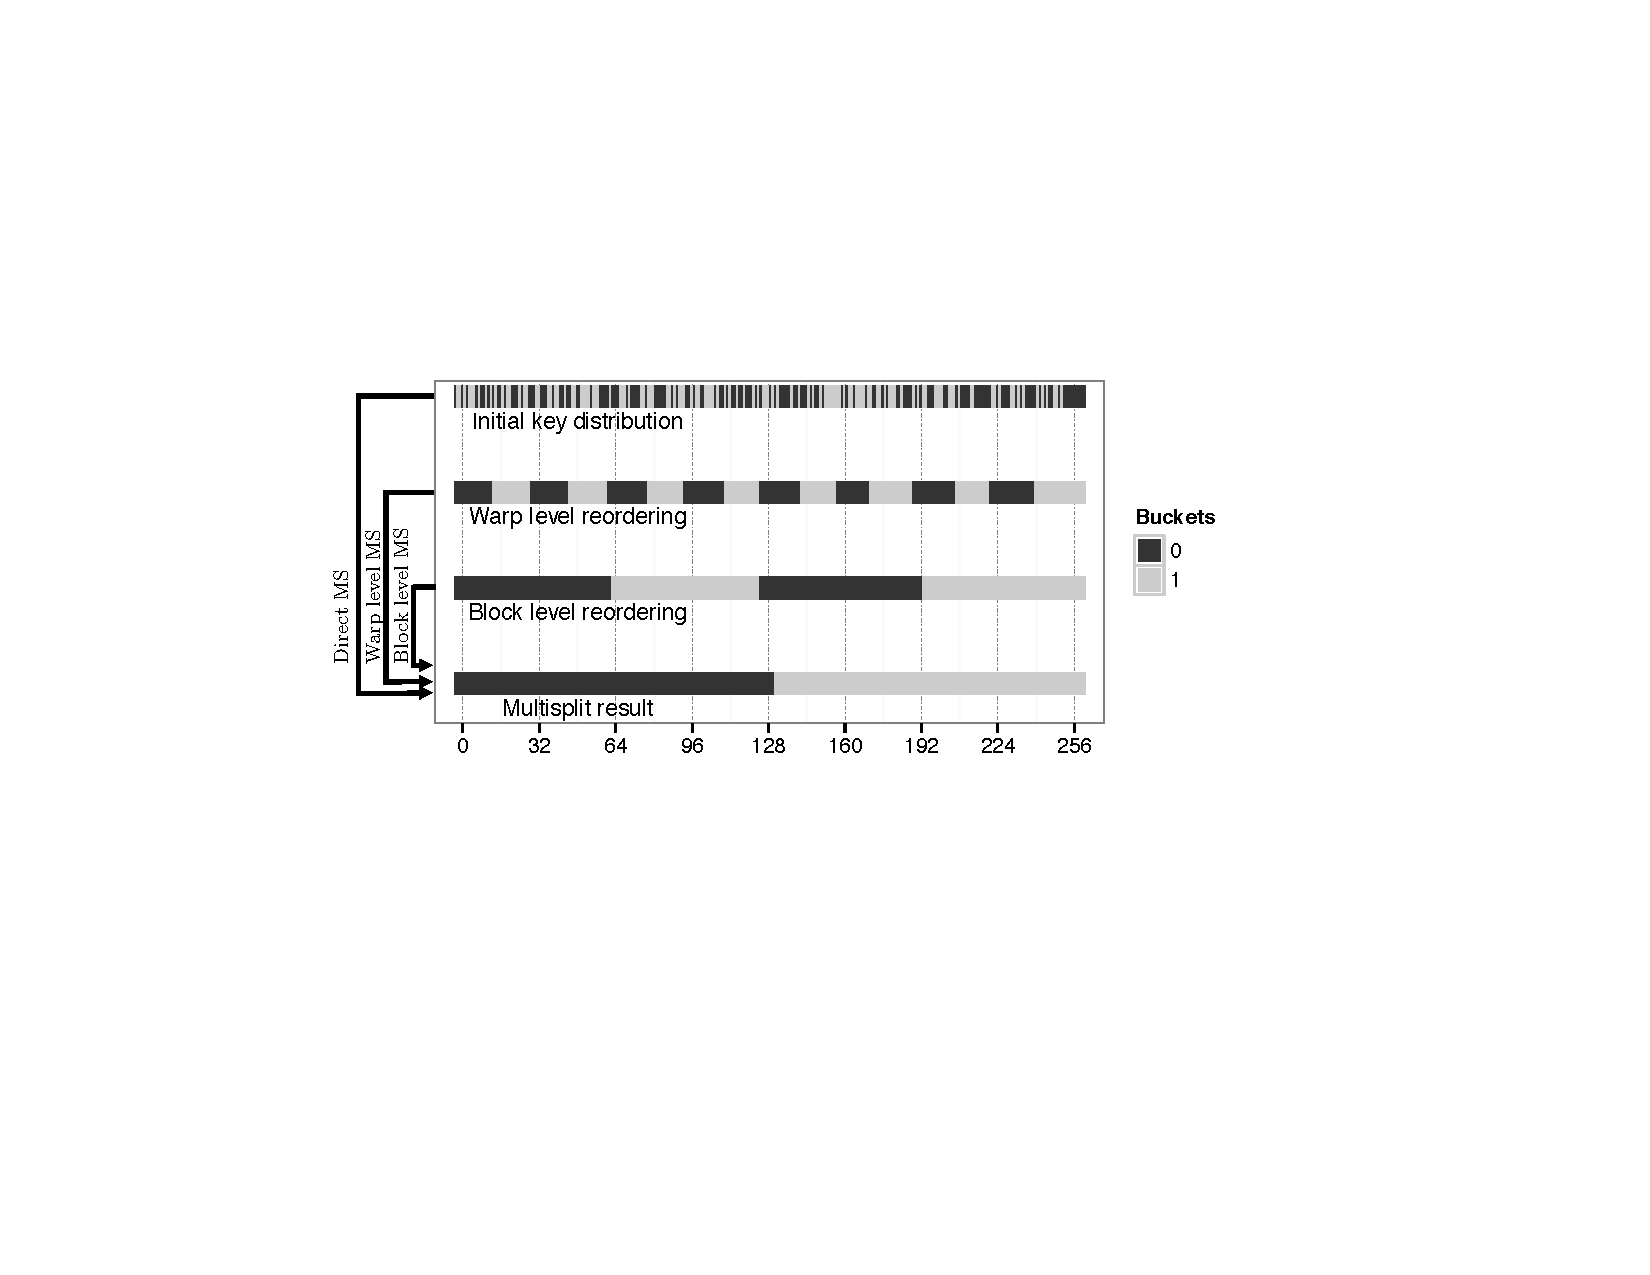
\includegraphics[width = 0.5\linewidth]{dist_2_mod.pdf}
        \label{fig:dist_2}
}
\subfloat[Key distribution with 8 buckets]
{
        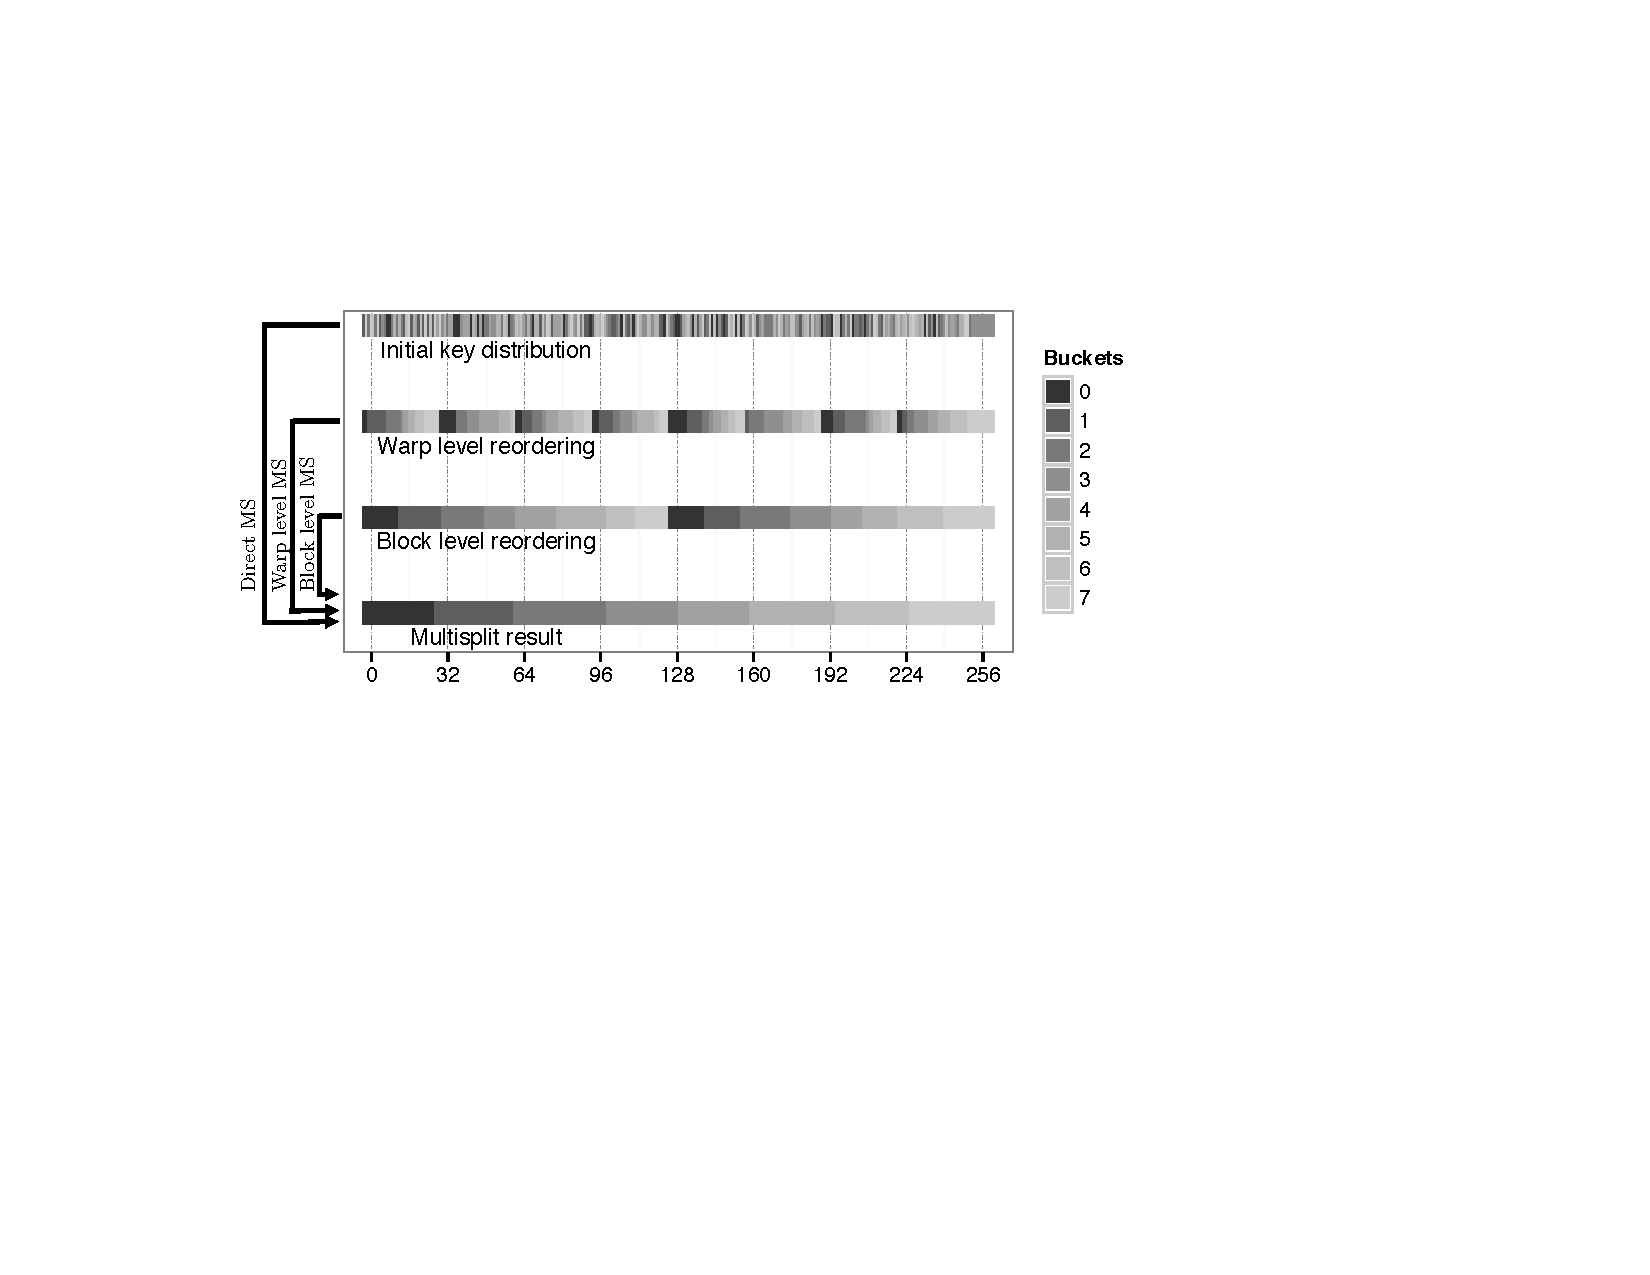
\includegraphics[width = 0.5\linewidth]{dist_8_mod.pdf}
        \label{fig:dist_8}
}
\caption{Key distributions for different multisplit methods and different number of buckets. Key elements are initially uniformly distributed among different buckets. This window shows an input key vector of length 256; each warp is 32 threads wide and each block has 128 threads. }\label{fig:dist}
\end{figure}

\subsubsection{Warp-level Reordering}\label{subsubsec:warp_reordering}
WMS extends DMS by reordering each tile (a group of consecutive windows in WMS) before the final write for better memory coalescing behavior.
Our first question was whether we prefer to perform the reordering in our pre-scan stage or our post-scan stage. We know that in order to compute the new index for each element in a tile, we need to know about its histogram and we need to perform a local (warp-level) exclusive scan over the results. We have already computed the warp level histogram in the pre-scan stage, but we do not have it in the post-scan stage and thus would either have to reload it or recompute it.

However, if we reorder key-value pairs in the pre-scan stage, we must perform two coalesced global reads (reading key-value pairs) and two coalesced global writes (storing the reordered key-value pairs before our global operation) per thread and for each key-value pair. Recall that in DMS, we only required one global read (just the key) per thread and per key in its pre-scan stage.

In the end, the potential cost of the additional global reads was significantly more expensive than the much smaller cost of recomputing our efficient warp-level histograms. As a result, we reorder in the post-scan stage and require fewer global memory accesses overall.

The main difference between DMS and WMS is in post-scan, where we compute both warp-level histogram and local offsets (Algorithm~\ref{alg:warp_histogram}~and~\ref{alg:warp_offsets}).
As we described before, in WMS each subproblem is divided into several tiles. Each tile is assigned to a warp and is processed in a consecutive number of windows of length 32 each.
Each warp, however, only performs reordering for all elements within a tile (not among all tiles).
This decision is mostly because of limited available shared memory per block.

Algorithms~\ref{alg:warp_histogram}~and~\ref{alg:warp_offsets} provide histogram and local offsets per window of read data. So, in order to perform warp-level reordering (performing a local multisplit within a tile), we need the following items to be computed for each key-value pair to be able to compute their new positions in shared memory:
\begin{enumerate}
        \item local offsets for each window (same tile, same bucket, same window)
        \item total number of elements processed by the same warp (same tile), from the same bucket, but from previous windows
        \item total number of elements in the same tile, but from previous buckets
\end{enumerate}
The first item is exactly the warp-level local offset computed in Section~\ref{subsubsec:warp_offset}.
The second item can be computed as follows: each thread within a warp directly computes all histogram results for all its windows. So, it can locally compute an exclusive scan of these results. However, each thread only has access to the counts per window of the  bucket for which it is in charge (i.e., the bucket equal to its lane ID). As a result, it is enough for each thread to ask for the appropriate value of~(2) by asking the thread who owns it (via a single shuffle instruction).

For the third item, we do the following: each thread within a warp has already computed the total number of elements per window (for specific buckets). So, it can easily add them together to form the histogram for all the windows (tile histogram).
All that remains is to perform another exclusive scan among these values such that each thread has the total number of items from previous buckets within the same tile.
This result too can be provided to threads by using a single shuffle instruction.
We can now perform reordering for key-value pairs into shared memory.

After performing the warp-level reordering, we need to write back results into global memory and into their final positions. To do so, all threads within a warp once again read key-value pairs from shared memory (it will be in $N_\text{window}$ coalesced reads).
Since items are reordered, previous threads are not necessarily reading the same items as before and hence they should identify their buckets once again.
Since elements are already reordered (consecutive elements belong to the same bucket), the new local offset among all other keys within the same bucket and same tile can be recomputed in a much easier way: each item's index (within shared memory) minus the offset computed in step (3)~of reordering (which can be accessed by a single shuffle instruction).
Finally we can add the computed local tile-offsets to the global offset offsets computed by the scan-stage, and perform final data movements in a (more likely) coalesced way.

\subsubsection{Block-level Reordering}\label{subsubsec:block_reordering}
The benefit from warp-level reordering is rather modest, particularly as the number of buckets grows, because we only see a small number of elements per warp (a WMS's tile) that belong to the same bucket. For potentially larger gains in coalescing, our BMS reorders entire blocks (larger tiles by a factor of $N_\text{warp}$).
That being said, an important advantage of our WMS is that almost everything can be computed within a warp, and since warps perform in lockstep, there will not be any need for further synchronizations among different warps.
In contrast, any coordination among warps within a thread-block requires proper synchronization.

As we mentioned before, each subproblem in BMS is assigned to a thread-block and is divided into several tiles. Each tile is assigned to multiple warps within a block. Each warp divides its share into multiple consecutive windows of 32 elements each.
Final positions can be computed in a hierarchical approach with 5 levels of localization, as described in equation~\ref{eq:permutation3}.

In BMS, although each block can process multiple consecutive tiles, we only perform reordering per tile (mostly because of limited available shared memory per block).
Reordering is equivalent to performing local multisplit over each tile. We can summarize the required computations for this reordering with the following two items:
\begin{enumerate}
        \item block-level local offsets
        \item total number of keys in the same tile, from previous buckets
\end{enumerate}
The first item can be computed as described in Section~\ref{subsubsec:block_offset}.
During the above computation, at some point we stored results from a segmented exclusive scan into shared memory.
Since our shuffle-based segmented scan is initially an inclusive scan, each thread has to subtract its initial bucket count from it to make it an exclusive scan.  
So, during that computation, with minimal extra effort, we could also store results for the sum of all elements within each segment (i.e., the total number of elements within each bucket in that tile) into another location in shared memory as well (for a total of $m$ elements). We refer to this result as our tile histogram.
Now, here each warp can reload the tile histogram from shared memory and perform a warp-wide exclusive scan operation on it.
In order to avoid extra synchronizations, every warp performs this step independently (as opposed to the option that a single warp computes it and puts it into shared memory, thus making it available for all other warps).
Thus, each thread can easily ask the required value for item~(2) by using a single shuffle instruction to fetch the value from the thread that owns that bucket's result.

After all threads within a block finish storing reordered key-value pairs into shared memory (for a single tile), we perform the final data movements.
Threads read the reordered tile (different key-value pairs than before), identify their buckets, and compute the final positions based on the following items:
\begin{enumerate}[label=(\roman*)]
        \item The new block-level local offset
        \item total number of elements from previous subproblems (the whole device) and from previous buckets
\end{enumerate}
Since elements are now already reordered, consecutive elements belong to the same bucket. As a result, the first item is equivalent to the index of that element (within shared memory) minus the starting index for that specific bucket (which is exactly item (2)~in reordering).
The second item is also already computed and available from our scan stage.
So, threads can proceed to perform the final data movement.
%%%%%%%%%%%%%%%%%%%%%%%%%%%%%%%%%%%%%%%%%%%%%%%%%%%%%%%%%%%%%%%%%%%
\subsection{More buckets than the warp width}\label{subsec:more_buckets}
\paragraph{Warp-level histogram and local offset computation}
Throughout the previous discussion, our primary way of computing a histogram in each warp (which processes a group of windows one by one) is to make each thread responsible to count the total number of elements with the bucket ID equal to its lane ID\@.
Since the current generation of GPUs has $N_\text{thread}=32$ threads per warp, if the number of buckets is larger than the warp width, we must put each thread in charge of multiple buckets (each thread is in charge of $\lceil m/32\rceil$ buckets as described in Section~\ref{subsubsec:warp_histogram}).
The total number of ballots required for our warp-level histogram procedure scales logarithmically ($\lceil\log m\rceil$).
Local offset computations are also as before (with $\lceil \log m\rceil$ ballots).

\paragraph{Block-level histogram and local offsets computations}
If $m>32$, besides the changes described above, to perform our segmented scan and reductions (Section~\ref{subsubsec:block_histogram}), 
each thread should participate in the computations required by $\lceil m/32\rceil$ segments.
% it requires that each thread must participate in the computations required for at most $\lceil m/32 \rceil$ segments.
Previously, for $m > 32$ buckets we used CUB's block-wide scan operation~\cite{Ashkiani:2016:GM}.
However, although CUB is a very efficient and high-performance algorithm in performing scan, it uses a lot of registers to achieve its goal. As a result, we prefer a more register-friendly approach to these block-level operations, and hence implemented our own segmented scan and reductions by simply iterating over multiple segments, processing each as described in Section~\ref{subsubsec:block_histogram} and Section~\ref{subsubsec:block_offset}.
%%%%%%%%%%%%%%%%%%%%%%%%%%%%%%%%%%%%%%%%%%%%%%%%%%%%%%%%%%%%%%%%%%%
\subsection{Privatization}\label{subsec:ms_privatization}
Traditionally, multisplit~\cite{He:2008:RJG} (as well as histogram and radix sort~\cite{Bell:2011:TAP,Merrill:2015:CUB} with some similarities) were implemented with a thread-level approach with thread-level memory \emph{privatization}: each thread was responsible for a (possibly contiguous) portion of input data.
Intermediate results (such as local histograms, local offsets, etc.) were computed and stored in parts of a memory (either in register or shared memory) exclusively dedicated to that thread.
Privatization eliminates contention among parallel threads at the expense of register/shared memory usage (valuable resources).
Memory accesses are also more complicated since the end goal is to have a sequence of memory units per thread (commonly known as \emph{vectorized} access), as opposed to natural coalesced accesses where consecutive memory units are accessed by consecutive threads. That being said, this situation can be remedied by careful pipelining and usage of shared memory (initially coalescing reads from global memory, writing the results into shared memory, followed by vectorized reads from shared memory).

In contrast, in this work, we advocate a \emph{warp-level} strategy that assigns different warps to consecutive segments of the input elements and stores intermediate results in portions of memory (distributed across all registers of a warp, or in shared memory) that are exclusively assigned to that particular warp~\cite{Ashkiani:2016:GM}.
An immediate advantage of a warp-level strategy is a reduction in shared memory requirements per thread-block (by a factor of warp-width).
Another advantage is that there is no more need for vectorized memory accesses, relieving further pressure on shared memory usage.
The chief disadvantage is the need for warp-wide intrinsics for our computations. These intrinsics may be less capable or deliver less performance. On recent NVIDIA GPUs, in general, using warp-wide intrinsics are faster than regular shared memory accesses but slower than register-level accesses.
A more detailed comparison is not possible since it would heavily depend on the specific task at hand.
However, efficient warp-wide intrinsics open up new possibilities for warp-wide computations as fundamental building blocks, allowing algorithm designers to consider using both thread and warp granularities when constructing and tuning their algorithms.
